\section{Additional material}
\label{sec:appendix}

\subsection{Optuna search spaces}

\begin{table}[H]
\centering
\caption{Search spaces of the three models. ``log'': sampled on a log scale.
$r = N_{\text{neg}}/N_{\text{pos}} \approx 3.18$ on the development set.}
\label{tab:search-spaces}
\small
\begin{tabular}{lll}
\toprule
Model (trials) & Hyperparameter & Range \\
\midrule
Logistic regression (25) & \code{C} & $[10^{-3}, 10]$, log \\
                         & \code{l1\_ratio} & $[0, 1]$ \\
                         & \code{class\_weight} & None or balanced \\
\midrule
Random forest (20) & \code{n\_estimators} & 100 to 300, step 50 \\
                   & \code{max\_depth} & 4 to 24 \\
                   & \code{min\_samples\_leaf} & 1 to 50, log \\
                   & \code{max\_features} & $[0.1, 0.6]$ (share of the columns) \\
                   & \code{class\_weight} & None or balanced \\
\midrule
LightGBM (50) & \code{n\_estimators} & 100 to 1000, step 50 \\
              & \code{learning\_rate} & $[0.01, 0.2]$, log \\
              & \code{num\_leaves} & 8 to 128, log \\
              & \code{min\_child\_samples} & 5 to 100, log \\
              & \code{subsample} & $[0.5, 1]$, applied at every iteration \\
              & \code{colsample\_bytree} & $[0.5, 1]$ \\
              & \code{reg\_lambda} & $[10^{-3}, 10]$, log \\
              & \code{scale\_pos\_weight} & $[1, r]$ \\
\bottomrule
\end{tabular}
\end{table}

\subsection{Exploratory figures}

\begin{figure}[H]
\centering
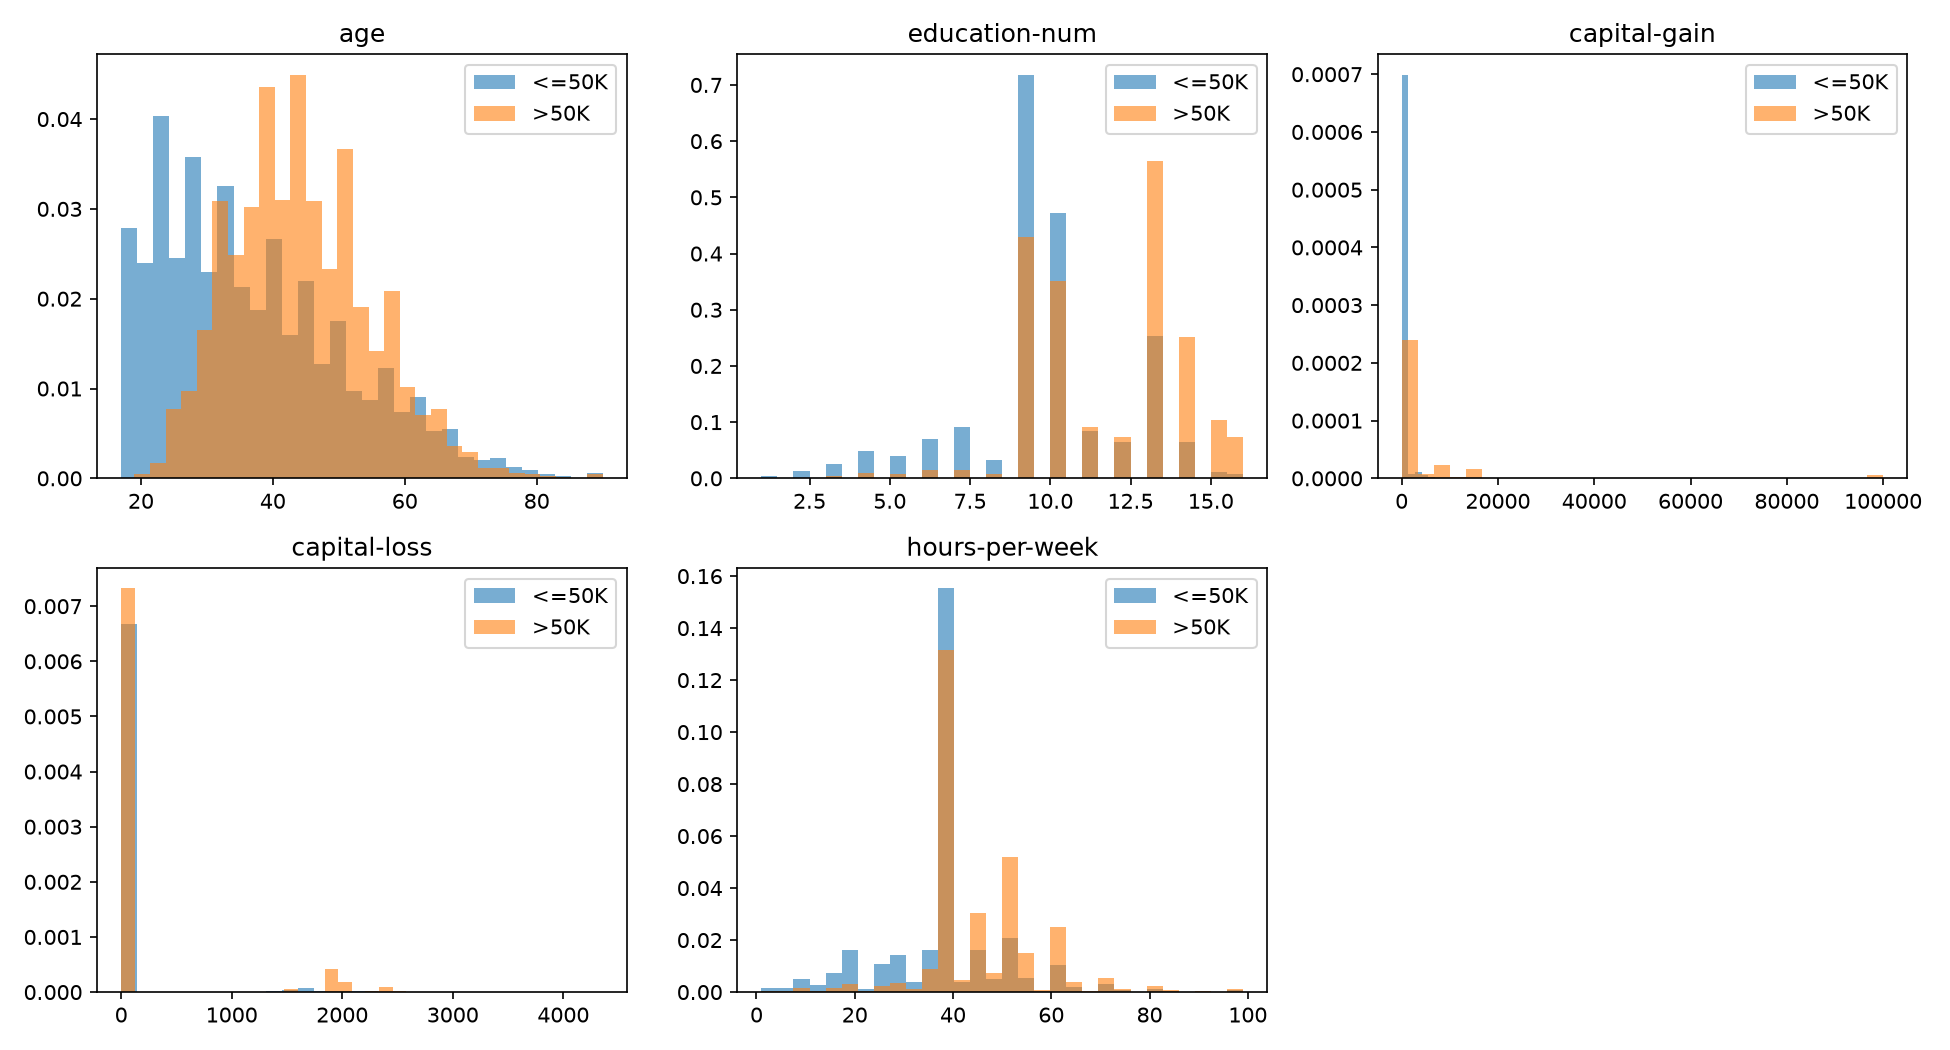
\includegraphics[width=0.95\textwidth]{eda_numeric_by_class.png}
\caption{Distribution of each numerical feature by class (development set,
densities).}
\label{fig:eda-numeric}
\end{figure}

\begin{figure}[H]
\centering
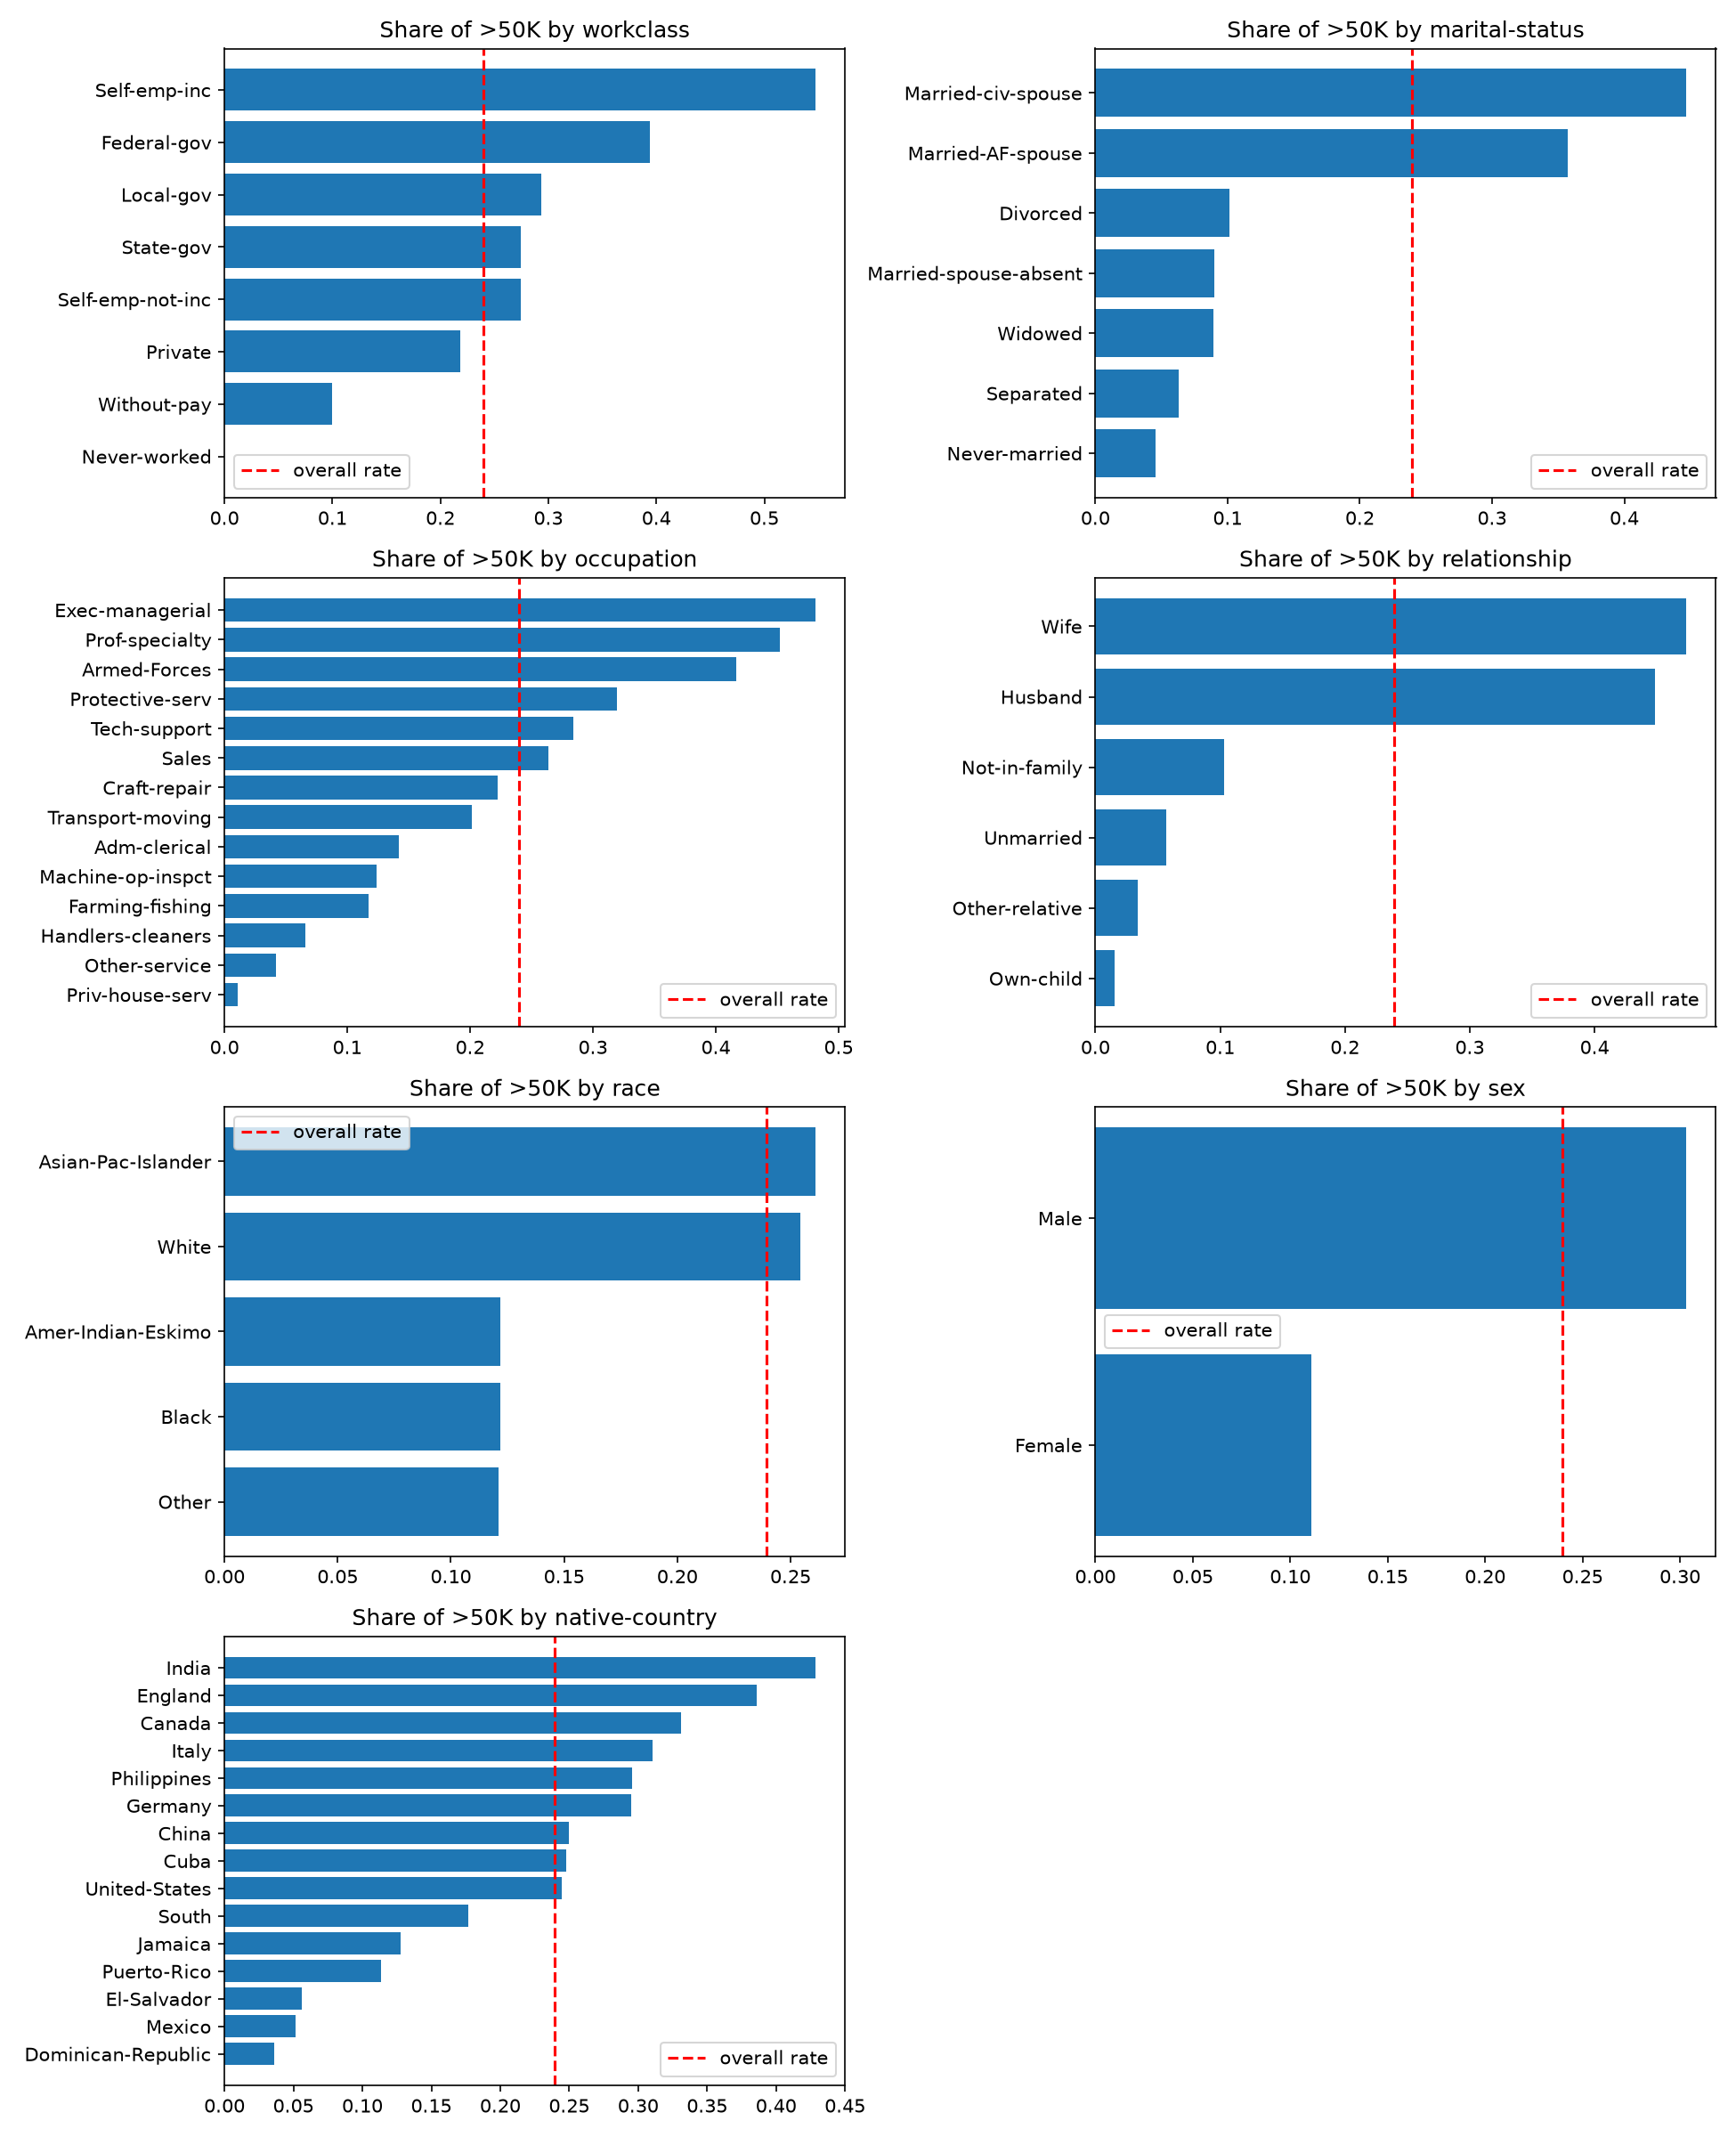
\includegraphics[width=0.85\textwidth]{eda_categorical_rates.png}
\caption{Share of \pos{} per category of each categorical feature (development
set). The dashed line is the overall share. For \code{native-country}, only the
15 most frequent countries are shown.}
\label{fig:eda-categorical}
\end{figure}
